\chapter{Methodology}\label{chap2}

\section{\textbf{Problem Statement}}

A road network can be considered an undirected graph $G = (V, E)$ where $V$ represents nodes, which is a collection of $N$ detector nodes, i.e., $V=\{v_1,v_2,...,v_n\}$ where $N = |V|$ and $v_i$ is the $i$th detector node. $E$ represents the $N_E = |E|$ road links connecting the detectors, and let $A \in \mathbb{R}^{N \times N}$ denote the adjacency matrix of $G$, i.e., $A = \{e_{ij}\}, i,j=1$ to $N$ where $e_{ij} = 1$ if nodes $v_i$ and $v_j$ are adjacent and $0$ otherwise.

Let each node of graph $G$ at time $t$ be represented by a $D$-dimensional feature vector represented as $\mathbf{x}_i^t \in \mathbb{R}^D$ that represents the node embeddings generated as explained later using node embeddings obtained from Node2Vec, other meta-information encoded, and traffic volume counts. Also, let the volume of traffic at time $t$ at node $i$ be $c_i^t$.

Define feature vectors for all nodes at a particular time $t$ as
\begin{equation*}
    \mathbf{X}_t = (\mathbf{x}_1^t, \mathbf{x}_2^t, \ldots, \mathbf{x}_N^t) \in \mathbb{R}^{N \times D} \tag{1}
\end{equation*}
Let the number of timesteps denoted by $T$ be a hyperparameter denoting the number of consecutive time steps under consideration. Then denote the values of all feature vectors over all nodes over $T$ consecutive time intervals starting at some time $t_0$ as
\begin{equation}
    \bm{\chi} = (\mathbf{X}_{t_0}, \mathbf{X}_{t_0+1}, \ldots, \mathbf{X}_{t_0+T-1}) \in \mathbb{R}^{T \times N \times D} \tag{2}
\end{equation}

Given the aforementioned notation, the problem that we are tackling in this paper can be formally defined as proposing a Traffic Digital Twin (TDT) that can perform the following tasks:
\begin{enumerate}[(i)]
    \item \textbf{Traffic prediction:} Given graph $G(V, E)$ and a sequence $\bm{\chi}$ of feature vectors of observed historical traffic flow over $T$ consecutive intervals, i.e., $\bm{\chi} = (\mathbf{X}_{t_0}, \mathbf{X}_{t_0+1}, \ldots, \mathbf{X}_{t_0+T-1})$, predict $\mathbf{Y}$, the traffic volume counts $c_i$ for $i \in N$ at the next timestep $t_0+T$, i.e., $\mathbf{Y} = \{c_1^{t_0+T}, c_2^{t_0+T}, \ldots, c_N^{t_0+T}\}$. Henceforth, we refer to this task as task (i).
    \item \textbf{Imputation:} Given graph $G(V, E)$ and a sequence $\bm{\chi}$ of feature vectors of observed historical traffic flow over $T$ consecutive intervals, i.e., $$\bm{\chi} = (\mathbf{X}_{t_0}, \mathbf{X}_{t_0+1}, \ldots, \mathbf{X}_{t_0+T-1})$$, a binary mask vector $\mathbf{M} \in \mathbb{R}^{N \times T}$ such that $\mathbf{M} = \{m_{ij}\}$ where $m_{ij} = 1$ if the traffic volume count at detector $i$ at time $t$ i.e. $c_{ij}$ is known and 0 otherwise to indicate its missing, impute the missing $c_{ij}$ values. Henceforth, we refer to this task as task (ii).
    \item \textbf{Traffic assignment on edge addition/removal:} Given original graph $G(V,E)$ and the new modified graph $G'(V', E')$ with an edge $e$ added or removed. Let $\phi$ be a hyperparameter denoting the number of closest neighbor nodes to the changed edge to mask out, i.e., $\mathbf{M} = \{m_i\}$ where $m_i = 1$ if the $\text{dist}(v_i,e)> \phi$ and 0 otherwise. Predict $\mathbf{Y'} = \{c'_1, c'_2, \ldots, c'_N \}$ where $c'_i$ is the traffic volume of the detectors with the modified topology $G'$. Henceforth, we refer to this task as task (iii).
\end{enumerate}

\section{\textbf{Data streaming framework}}

Reliable real-time data collection is a crucial aspect and prerequisite of a digital twin to effectively update internal parameters and synchronize with the real world. The Traffic Digital Twin (TDT), \modelname, presented in this paper requires real-time traffic volume data as input. We aim to use absolute traffic volume counts available at a manageable low frequency of 15 minutes to one hour. While systems with more sophisticated data at a higher frequency can be proposed, we aim to keep the real-world collection infrastructure cheap, simple, and based on already existing systems around the world. In particular, we strive to cater to the following objectives:

\begin{enumerate}[(i)]
    \item Hardware infrastructure should be cheap and easily replaceable.
    \item Easily extendable to use a variety of different sources.
    \item Should work with only absolute traffic counts, no other specific information like direction and vehicle types.
    \item Should work with a medium-frequency update.
\end{enumerate}

There are various possible ways to collect the type of data mentioned. The most reliable would be to install inductive loop detectors embedded in road surfaces at city intersections. Such systems are already available and in use in several major cities. For example, the Sydney Coordinated Adaptive Traffic System (SCATS)\cite{scats} is available in over 180 cities across 28 countries, including New Zealand, Dublin, Shanghai, and Hong Kong \cite{wiki:sydney_traffic_system}. New York City's Adaptive Traffic Control System (ATCS), Adaptive Signal Control Technology (ASCT), SCOOT, and ACS are other such systems that are used to control traffic signal timings and optimize congestion. Such systems can be easily extended to use with our proposed model since we only use absolute traffic volume counts, which such systems are capable of collecting.

Another possible data source can be surveillance cameras assisted with computer vision models\cite{jain2019review}, which is already used in practice at some intersections in Shenzhen, China. Several existing studies\cite{asha2018vehicle} using state-of-the-art object detection models like YOLO\cite{redmon2018yolov3} demonstrate the effectiveness of this method. Such a model-based approach allows for cheap and effective traffic monitoring on top of existing surveillance camera infrastructure. 

Other methods like using GPS-enabled mobile phones\cite{rose2006mobile} to track urban traffic flow, as Google does in its Maps product, and the use of probe vehicles\cite{zhu2012probe}, which are vehicles equipped with detectors that may be taxis or public transport, can also be used to approximate traffic volume based on their data.

We aim for our model to work in conjunction with multiple data streams, as different parts of the road network may be served with different data sources. We want our TDT to seamlessly integrate with these sources, so we need an aggregator of sorts to reconcile the data from the different streams and store them in a data lake. This data can then be used by the TDT model to keep its internal state in sync with real-world data.

The deployed aggregator system will have an RPC and API interface that can be interacted with by the remote sensors and other data sources. Each different service can have a separate interface built to interact with the aggregator service. The aggregator then stores all the data with relevant meta information in a datalake which is a centralized repository that allows you to store all your structured and unstructured data. We make use of a datalake as different sources might have additional information apart from just traffic volume counts, and by allowing us to store other complementary information, we leave possible avenues for building up further capabilities in our TDT.

An example representing a simplified view of the aforementioned process is shown in Fig. \ref{fig:framework}.

\begin{figure*}[t]
  \centering
  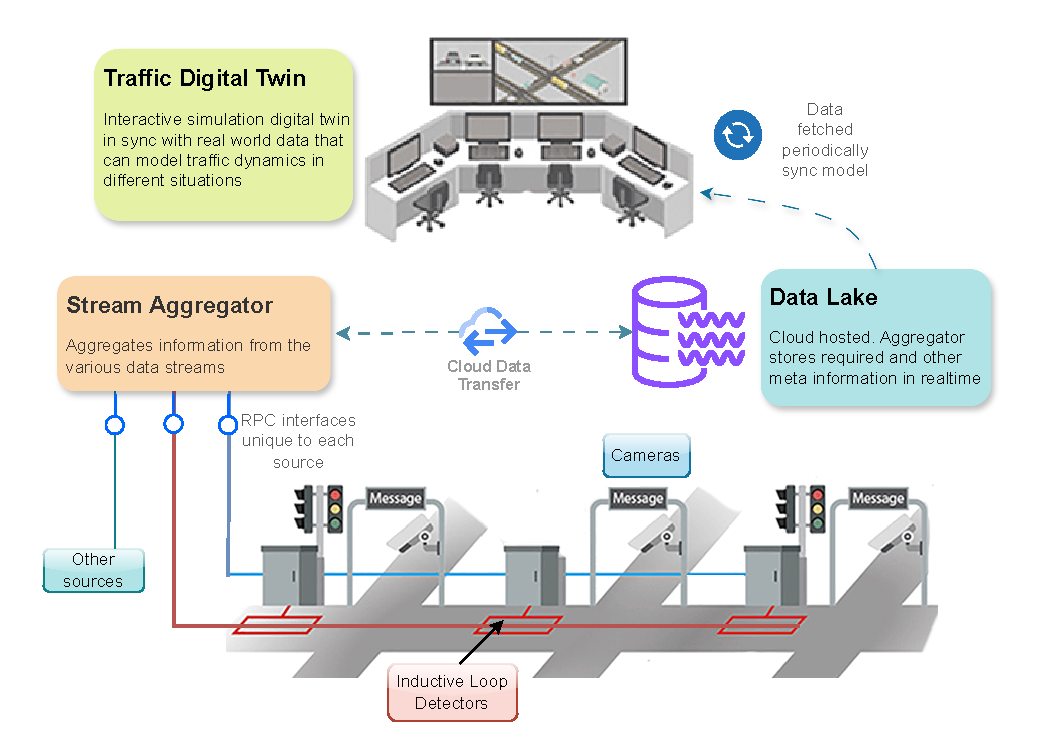
\includegraphics[width=1\textwidth]{images/framework.pdf} % Adjust width as needed
  \caption{Traffic Digital Twin (TDT) data processing}
  \label{fig:framework}
\end{figure*}

\section{\textbf{Model input}}

For each node, we create a feature vector that represents all the information related to that node. The feature vector for a node is composed of three feature vectors that are, as defined ahead, concatenated:

\subsection{Graph embedding generation using Node2Vec:}

In order for the model to effectively learn the spatial relationships between the detector nodes based on graph structure, we need a way to generate an appropriate representation of the graph nodes that capture the neighborhood structure effectively. $Node2Vec$\cite{node2vec} is a feature learning algorithm that uses second-order biased random walks in a Skip-gram architecture to learn feature vectors for nodes in the graph. There are two key steps for feature generation:

\begin{enumerate}[(i)]
    \item \textit{Sampling using second-order biased random walks}: Two hyper-parameters \( p \) and \( q \) are introduced, which are the "return" and "in-out" parameters, respectively. Suppose we simulate a random walk of fixed length \( l \). Let \( c_i \) denote the \( i \)th node in the walk, starting with \( c_0 = u \). Nodes \( c_i \) are generated by the following distribution:
    \[
        P(c_i = x \mid c_{i-1} = v) =
        \begin{cases}
        \frac{\pi_{vx}}{Z} & \text{if } (v,x) \in E \\
        0 & \text{otherwise}
        \end{cases}
    \]
    where \( \pi_{vx} \) is the unnormalized transition probability between nodes \( v \) and \( x \), and \( Z \) is the normalizing constant.
    
    For a walk that just traversed edge \( (t,v) \) and now resides at node \( v \), we now need to decide on the next step so it evaluates the transition probabilities \( \pi_{vx} \) on edges \( (v,x) \) leading from \( v \). The transition probability \( \pi_{vx} = \alpha_{pq}(t,x)\cdot w_{vx} \), where 
    \[
        \alpha_{pq}(t,x) = 
        \begin{cases}
        \frac{1}{p}  & \text{if } d_{tx} = 0\\
        1 & \text{if } d_{tx} = 1\\
        \frac{1}{q} & \text{if } d_{tx} = 2
        \end{cases}
    \]
    and \( d_{tx} \) denotes the shortest path distance between nodes \( t \) and \( x \).

    \item \textit{Optimizing objective function using Skip-gram}: Let for graph \( G(V, E) \), \( f: V \rightarrow \mathbb{R}^d \) be the \( d \)-dimensional feature representation function. Thus, \( f \) is a matrix of size \( |V| \times d \) parameters. Now, for every node \( u \in V \), we define \( N_S(u) \subset V \) as a \emph{network neighborhood} of the node \( u \) generated in step (i). Define similarity between two nodes \( u \) and \( v \) as:
    \[
        P_f(v|u) = \frac{\exp(f(v)^T f(u))}{\sum_{w \in V} \exp(f(w)^T f(u))} \tag{1}
    \]
    For neighborhood \( N_s(v) \) of \( v \), define the probability of the neighborhood of \( u \) as:
    
    \[ P_f(N_s(u)|u) = \prod_{v \in N_s(u)} P_f(v|u) \tag{2} \]

    Further, the global neighborhood likelihood for a given \( f \) can be define as:
    \[ \sum_{u \in V} \log P_f(N_s(u)|u) \tag{3}\]
    which is the objective function that we want to maximize through the feature representation function \(f\). Hence,
     \[
    \max_{u \in V} \sum_{u \in V} \log \left( \prod_{v \in N_s(u)} \frac{\exp(f(v)^T f(u))}{\sum_{w \in V} \exp(f(w)^T f(u))} \right) \tag{4}
    \]
\end{enumerate}

\begin{figure*}[t]
  \centering
  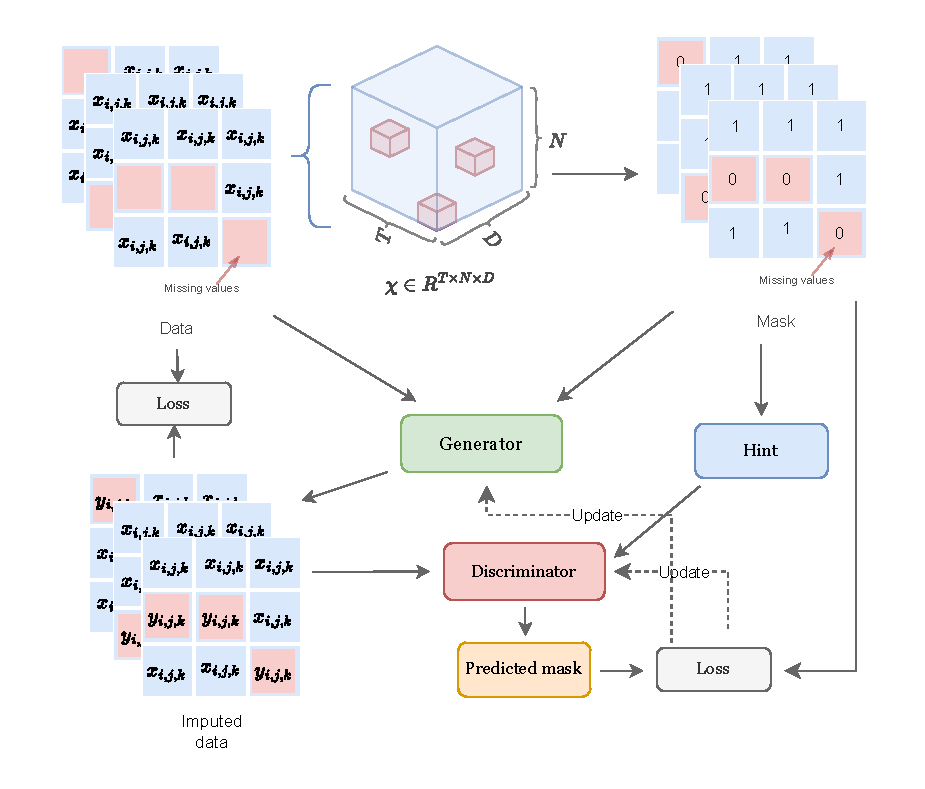
\includegraphics[width=1\textwidth]{images/model.pdf}
  \caption{Model architecture}
  \label{fig:dataset}
\end{figure*}

\subsubsection{Traffic volume normalised:}
The input data should be normalized to increase the training speed and effectiveness. The traffic volume counts at different detectors are normalized as follows:
\[
x_{\text{norm}} = \frac{x - x_{\text{min}}}{x_{\text{max}} - x_{\text{min}}}
\]
Thus, \( x_{\text{norm}} \) is in the range \([0,1]\) after normalization. This same approach is used for other continuous or discrete single-valued features.

\subsection{Word2Vec encoding of other exogenous variables:}
Skip-gram\cite{skipgram}, a popular Word2Vec\cite{word2vec} architecture, aims to predict the context words given a target word. It learns to encode the semantic meaning of words by maximizing the probability of context words given the target word. Mathematically, the objective function for Skip-gram can be represented as:

\[
J_\theta = \frac{1}{T}\sum^{T}_{t=1}\sum_{-n\leq j \leq n, j \neq 0}\log p\left(w_{j+1} \mid w_{t}\right)
\]

where \( w_t \) represents the target word at position \( t \), \( c \) is the size of the context window, and \( T \) is the total number of words in the corpus.

We use \textit{Word2Vec} to encode the other possibly relevant exogenous variables, like weather, road type, etc., as features to the model input, thus increasing its effectiveness. We would like to note that this approach is easily extensible to any number of other features that may prove to be relevant in the future, and we wish to add them to the model input.

\vspace{3ex} Concatenating the feature vectors from the above sub-parts, we get the final input vector. Extending the notation as defined in section III.A, for \(N\) nodes, we define the construction of \(\mathbf{x}_i^t\), the feature vector of the node \(i\) at time \(t\). Assuming \textit{Node2Vec} was used as defined in (i) to generate \(R^{D_g}\) dimensional graph embeddings for each node. Let \(g_i\) be the graph embedding for node \(i\). Then, for \(n\) single-dimensional real-valued features \((r_1, r_2, \ldots, r_n)\), let them be normalized as defined in (ii) to \((r_1^{\text{norm}}, r_2^{\text{norm}}, \ldots, r_n^{\text{norm}})\) thus creating a \(D_n = n\) dimensional vector. Let them be represented by \(h_i^t\). Finally, for \(m\) "words" representing other semantic information related to the node, and using \textit{Word2Vec} to output \(d_w\) dimensional vectors for each word, we get a \(R^{mxd_w}\) dimensioned vector that we flatten and represent as \(k_i^t\) \(\in\) \(R^{D_w}\) where \(D_w = m \times d_w\).

Finally, one concatenation of the above three, we get the feature vector of node \(i\) at time \(t\) 
\[\mathbf{x}_i^t = (\ g_i\ ||\ h_i^t\ ||\ k_i^t\ ) \in R^D\] 
where \(D = D_g+D_n+D_w\).
Thus, from (i) and (ii), over \( T \) consecutive time steps and for \( N \) nodes, we get the final feature vector as \( \mathbf{\chi} \)  \(\in\) \( \mathbb{R}^{T \times N \times D} \).
Depending on the task, we also add other task-specific inputs, like, for the case of imputation, a binary matrix \( M \) representing the missing and known values. Specific implementation details are discussed further in the experiments section.

\section{\textbf{Physics Informed Deep Learning}}

Physics-informed deep learning (PIDL) represents a distinct approach within deep learning (DL), where a neural network is trained to tackle learning tasks while adhering to the principles of physics. By integrating fundamental physical laws as prior knowledge, the resulting neural network serves as a data-efficient approximator, adept at processing input data and delivering accurate predictions.

In situations where systems are required to adhere to the physical laws, PIDL is especially useful as it biases the model to follow the physics models; this allows the model to generate more accurate results, specially GANs, as this eliminates several possible predicted distributions that are not viable do to not adhering to the physical laws of the system.

In our situation, specifically with problem 3. of Traffic assignment on edge addition/removal, where we have to predict the changed volume counts on the same timestep but with modified topology, it is imperative, according to the \textit{conservation law} of traffic, that in such a case that the total volume of traffic in a large enough region prior to and after redistribution will be same.

Formally, for a particular fixed time, let \( G(V, E) \) be the original graph, and \( G'(V', E') \) be the graph obtained by adding or removing an edge \( e \). Similarly, \( c_i \) represents the traffic volume at detector \( i \) in \( G \) for \( i = 1 \) to \( N = |V| \), and \( c_i' \) represents the traffic volume at detector \( i \) in \( G' \) for \( i = 1 \) to \( N' = |V'| \). Then from \textit{conservation law}:
\begin{equation}
    C = \sum_{i=1}^{N} c_i = C' = \sum_{i=1}^{N'} c'_i \tag{5}
\end{equation}

In order to bias the model for conservation as described in Eq. (3), it needs to be integrated into the learning process of the PIDL network. The simplest way to do it is to define it as an additional term to the loss used to update the model, basically penalizing the model heavily for predictions that do not conform to the physical constraints. With traffic volumes \(c_i\) along with other graph information as training input, we establish two different measures for the Discriminator to evaluate generator output:
\begin{enumerate}
    \item \textbf{\( \mathcal{L}_{DL} \)}: Denoting the conventional discriminator loss defined as:
    \[ \mathcal{L}_{DL} = \mathbb{E}_{x \sim P_{\text{data}}}[D(x)] - \mathbb{E}_{z \sim P_z}[D(G(z))] \]

    \item \textbf{\( \mathcal{L}_{PHY} \)}: Denoting the conservation loss. As defined in Eq. (3), for a given mask \( M \), let \( S \) be the set of detectors such that \( M(i) = 0 \), specifically \( S = \{i \mid M(i) = 0\} \). Then let \( C_0 \) be the sum of masked traffic volume counts, i.e., \( C_0 = \sum_{i \in S} c_i \), and \( Y = \{c'_i \mid i \in S\} \) be the generator output. Then define:
    \[ \mathcal{L}_{PHY} = (C_0 - \sum_{i \in S} c'_i)^2 \]
\end{enumerate}
In order to control the dominance of the different components of the loss function, we introduce two new hyperparameters, \( \mu \) and \( \lambda \), to adjust the weights of \( \mathcal{L}_{DL} \) and \( \mathcal{L}_{PH} \) respectively. Thus, the final loss function can be defined as:

\[ \mathcal{L} = \mu \cdot \mathcal{L}_{DL} + \lambda \cdot \mathcal{L}_{PHY} \]

In conclusion, by leveraging hyperparameters, we can fine-tune the model's balance between different objectives. Biasing the Discriminator to respect physical laws allows the generator to better capture underlying patterns in the data, a capability we found useful in our experiments, as we describe ahead.

\section{\modelname: Traffic Model}

In this section, we present the architecture of our \modelname\ model, which is inspired by architectures of Generative Adversarial Imputation Nets (GAIN)\cite{gain} and Wasserstein Generative Adversarial Network (WGAN)\cite{wgan}. GAIN is a new and popular type of conditional GAN that has been applied to a variety of missing value imputation tasks on different datasets with favorable results. WGAN is an improvement over traditional GANs proposed by M. Arjovsky et al., that is designed to improve training stability by focusing on using Wasserstein distance metric instead of the traditional Jensen-Shannon divergence, along with some other architecture changes like gradient clipping, removal of sigmoid, etc., that have been shown to result in more reliable convergence and better quality samples.

\subsection{\textit{Generator:}}

The generator \( G \) accepts inputs of observed data with missing values, denoted by \( \mathbf{X} \), the binary mask vector \( \mathbf{M} \), which indicates what the missing values and a noise vector denoted by \( \mathbf{Z} \) are. It produces imputed data \( \mathbf{X}_g \), representing a vector of imputations, which is then projected to form the complete imputed output \( \mathbf{Y}_0 \). 

Formally, the output of the generator \( G \) can be denoted as: 
\[ \mathbf{X}_g = G(\mathbf{X}, \mathbf{M}, (\mathbf{1}-\mathbf{M}) \odot \mathbf{Z}) \]

where \( \odot \) denotes the Hadamard product or the element-wise multiplication and \( \mathbf{Z} \) is the \( d \)-dimensional noise vector. \( \mathbf{X}_g \) represents the missing values which are then filled back in \( \mathbf{X} \) as per the mask \( \mathbf{M} \), and this makes the final generator output that is then passed off to the Discriminator to judge.

\subsection{\textit{Discriminator:}}

Similar to the Discriminator in traditional GANs, we also use another model called the Discriminator, denoted by \( D \), that acts as an adversary to the Generator \( G \) and trains it. The discriminator \( D \), defined in the original GAIN implementation as \( D: \mathbf{\chi} \rightarrow [0,1]^d \), outputs a binary vector instead of a single real value, which denotes what components of the generator input are real (observed) and what are fake (imputed). 

So, in contrast to the traditional Discriminator used in GANs, which predicts whether the generated result is entirely fake or real, the Discriminator in GAIN predicts what components are real or fake. The loss, which is then used in SGD, is the mean of losses for individual components.

\subsection{\textit{Hint}}
GAIN introduces a new concept called the hint mechanism, represented by a random variable \( \mathbf{H} \) taking values in a space \( \mathcal{H} \). The aim of this hint mechanism is to provide additional missing information about the mask to the Discriminator. The following proposition was introduced and proved in the GAIN\cite{gain} original paper:

\begin{mdframed}[linewidth=0.5pt]
\textit{
\newtheorem{proposition}{Proposition}
\begin{proposition} \label{prop:nonunique}
    There exist distributions of \( \mathbf{X} \), \( \mathbf{M} \), and \( \mathbf{H} \) for which solutions to \( \hat{p}(\mathbf{x} | \mathbf{h}, m_i = t) = \hat{p}(\mathbf{x} | \mathbf{h}) \) for each \( i \in \{1, \ldots, d\} \), \( \mathbf{x} \in \mathcal{X} \), and \( \mathbf{h} \in \mathcal{H} \) such that \( p_h(\mathbf{h} | m_i = t) > 0 \) are not unique under the optimality criterion of GAN.
    \vspace{20pt}
\end{proposition}
}
\end{mdframed}

This means that there may exist several possible distributions that \( G \) may generate that may seem valid to \( D \), so \( \mathbf{H} \) must provide enough information to uniquely identify the correct representation of the underlying data, which is what the hint mechanism aims to do.

The hint mechanism depends on the binary mask vector \( \mathbf{M} \), and for each imputed sample \( (\hat{\mathbf{x}}, \mathbf{m}) \), we draw \( \mathbf{h} \) from the distribution \( \mathbf{H} | \mathbf{M} = \mathbf{m} \). We then add \( \mathbf{h} \) as an extra input to the Discriminator, resulting in a function \( D: \mathcal{X} \times \mathcal{H} \rightarrow [0, 1]^d \), where each component of \( D(\hat{\mathbf{x}}, \mathbf{h}) \) represents the probability that the corresponding component of \( \hat{\mathbf{x}} \) was observed given \( \hat{\mathbf{X}} = \hat{\mathbf{x}} \) and \( \mathbf{H} = \mathbf{h} \).
By varying how \( \mathbf{H} \) is defined, we control the level of information it provides about \( \mathbf{M} \).

\textcolor{gray!80}{\vrule width 0.95\columnwidth height 0.001pt depth 0pt \relax}

\vspace{1ex}

Finally, we take inspiration from the architecture of WGAN and incorporate some of those changes in our model. Traditional GANs suffer from training instability and model collapse, i.e., the inability to learn the diverse representations and only generate repetitive samples. Wasserstein GAN (WGAN), proposed by M Arjovsky et al., solves these problems, and we highlight some of the architectural changes we made to GAIN based on WGAN in the following paragraphs.

In traditional GAN, the generator and Discriminator are trained using the following loss functions:
\[
\mathcal{L}_{\text{GAN}}^G = \log(1 - D(G(z)))
\]
\[
\mathcal{L}_{\text{GAN}}^D = -\log(D(x)) - \log(1 - D(G(z)))
\]

Meanwhile, in WGANs, we remove the logarithms and use Wasserstein distance for loss instead.
\[
\mathcal{L}_{\text{WGAN}}^G = -D(G(z))
\]
\[
\mathcal{L}_{\text{WGAN}}^D = D(G(z)) - D(x)
\]

Another change in WGANs that we incorporate in GAIN is the absence of a sigmoid activation function in the Discriminator's output layer, unlike in traditional GANs. This alteration enables the Discriminator to output unbounded real-valued scores instead of probabilities. Additionally, WGANs incorporate gradient clipping as a regularization technique to enhance training stability. Gradient clipping involves setting a threshold value for the gradients, and if they exceed this threshold, they are scaled down to ensure that their magnitude does not surpass it. This approach helps stabilize the training process and mitigates issues such as exploding gradients.